\begin{frame}[t]{VERA Problem 4}
    
\begin{columns}
    \begin{column}{0.5\textwidth}
        \begin{itemize}
            \item Center 3x3 assembly cluster in Watts Bar Unit 1
            \item AIC Control rod in center assembly placed at 257.9 cm
            \item Test cases used 57 planes, with rod inserted 50\% into a plane
            \item Reference used 58 planes, with extra plane boundary aligned 
            with rod tip
            \item All simulations used 1 core per plane
        \end{itemize}
    \end{column}
    \begin{column}{0.28\textwidth}
        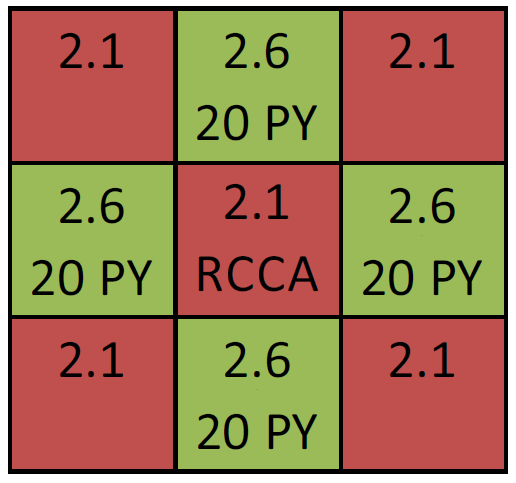
\includegraphics[width=\textwidth]{p4a_layout.png}
    \end{column}
    \begin{column}{0.22\textwidth}
        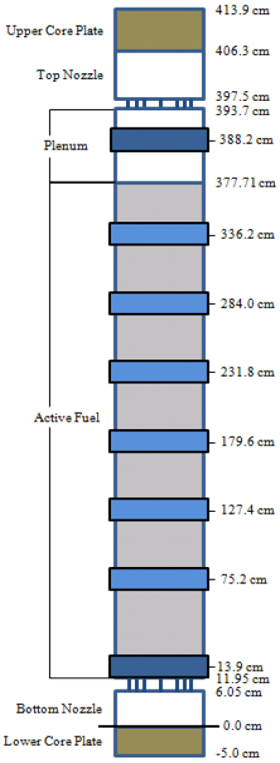
\includegraphics[width=\textwidth]{wb_3d_assembly.png}
\end{column}
\end{columns}
    
\end{frame}

%%%%%%%%%%%%%%%%%%%%%%%%%%%%%%%%%%%%%%%%%%%%%%%%%%%%%%%%%%%%%%%%%%%%%%%%%%%%%%%%%

\begin{frame}[t]{Problem 4 Results}
    
    \begin{table}[h]
      \centering
      \resizebox{\textwidth}{!}{
        \begin{tabular}{|c|c|c|c|c|c|c|}\hline
          \multirow{2}{*}{Case} & k-eff & \multicolumn{2}{|c|}{Pin Power Differences} & \multicolumn{2}{|c|}{Iterations} & Runtime\\\cline{3-6}
          & Difference (pcm) & RMS & Max & 2D/1D & CMFD & (Core-Hours) \\\hline
          Reference        & -- & --     & --      & 12 & 364 & 8.59 \\\hline
          No Treatment     & -30 & 3.84\% & 21.81\% & 12 & 352 & 9.23 \\\hline
          Polynomial       & -8  & 1.03\% &  6.58\% & 12 & 360 & 9.50 \\\hline
          Sub-plane         & -7  & 1.13\% &  7.11\% & 12 & 409 & 9.26 \\\hline
          Sub-plane + 1D-CP & -2  & 0.54\% &  4.94\% & 12 & 364 & 9.45 \\\hline
        \end{tabular}
      }
    \end{table}
    \begin{itemize}
        \item Maximum error for all cases occurs in pins neighboring the partially rodded pin cell
    \end{itemize}
    
\end{frame}

%%%%%%%%%%%%%%%%%%%%%%%%%%%%%%%%%%%%%%%%%%%%%%%%%%%%%%%%%%%%%%%%%%%%%%%%%%%%%%%%%

\begin{frame}[t]{VERA Problem 5}
    
    \begin{itemize}
      \item Bank D inserted to 257.9 cm, other banks all out
      \item 57 planes for tests and 58 for reference, 16 cores per plane
    \end{itemize}
    \begin{figure}[h]
      \centering
      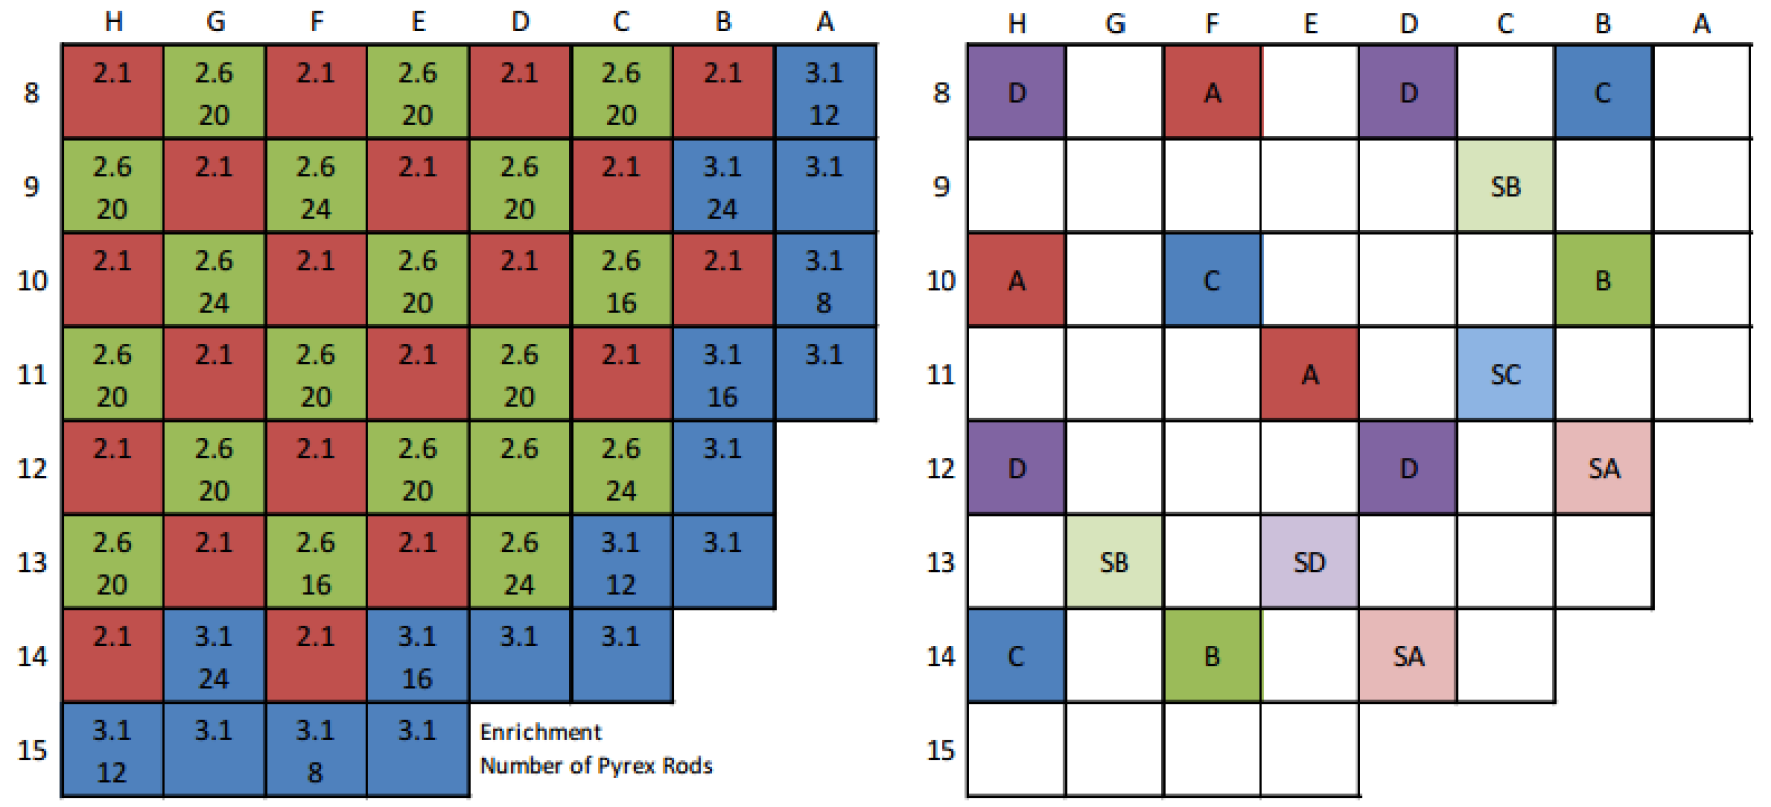
\includegraphics[width=0.9\textwidth]{WB1-cycle1-layout.png}
    \end{figure}
    
\end{frame}

%%%%%%%%%%%%%%%%%%%%%%%%%%%%%%%%%%%%%%%%%%%%%%%%%%%%%%%%%%%%%%%%%%%%%%%%%%%%%%%%%

\begin{frame}[t]{Problem 5 Results}
    
    \begin{table}[h]
      \centering
      \resizebox{\textwidth}{!}{
        \begin{tabular}{|c|c|c|c|c|c|c|}\hline
          \multirow{2}{*}{Case} & k-eff & \multicolumn{2}{|c|}{Pin Power 
          Differences} & \multicolumn{2}{|c|}{Iterations} & Runtime\\\cline{3-6}
          & Difference (pcm) & RMS & Max & 2D/1D & CMFD & (Core-Hours) \\\hline
          Reference         & --  & --     & --      & 13 & 481 & 362 \\\hline
          No Treatment      & -22 & 6.90\% & 30.55\% & 13 & 523 & 411 \\\hline
          Polynomial        & -5  & 1.15\% &  4.85\% & 13 & 463 & 374 \\\hline
          Sub-plane         & -5  & 2.09\% & 10.20\% & 13 & 499 & 399 \\\hline
          Sub-plane + 1D-CP & -1  & 0.50\% &  2.74\% & 13 & 529 & 426 \\\hline
        \end{tabular}
      }
    \end{table}
    \begin{itemize}
        \item Maximum error for each comparison occurs in pins neighboring the partially rodded pin cell
    \end{itemize}
    
\end{frame}